\documentclass[11pt,a4paper]{article}

% -------------------------------------------------
% ENCODAGE / LANGUE
% -------------------------------------------------
\usepackage[utf8]{inputenc}
\usepackage[T1]{fontenc}
\usepackage[french]{babel}

% -------------------------------------------------
% MISE EN PAGE
% -------------------------------------------------
\usepackage[a4paper,margin=2.5cm]{geometry}
\usepackage{setspace}
\usepackage{parskip}

% -------------------------------------------------
% MATHS / IMAGES / TABLEAUX
% -------------------------------------------------
\usepackage{amsmath,amssymb}
\usepackage{graphicx}
\usepackage{booktabs}
\usepackage{array}
\usepackage{float}

% -------------------------------------------------
% LIENS
% -------------------------------------------------
\usepackage[colorlinks=true,linkcolor=black,urlcolor=blue,citecolor=black]{hyperref}

% -------------------------------------------------
% CODE (optionnel)
% -------------------------------------------------
\usepackage{xcolor}
\usepackage{listings}
\renewcommand{\lstlistingname}{Code}

\definecolor{backcolour}{rgb}{0.95,0.95,0.95}
\definecolor{codegreen}{rgb}{0,0.5,0}
\definecolor{codegray}{rgb}{0.4,0.4,0.4}

\lstdefinestyle{mystyle}{
    backgroundcolor=\color{backcolour},
    commentstyle=\color{codegreen},
    numberstyle=\tiny\color{codegray},
    basicstyle=\ttfamily\small,
    breaklines=true,
    numbers=left,
    numbersep=5pt,
    showstringspaces=false
}

\lstset{
    basicstyle=\ttfamily\scriptsize,
    backgroundcolor=\color{gray!10},
    frame=single,
    breaklines=true,
    captionpos=b
}

\lstset{
  literate=
  {á}{{\'a}}1 {é}{{\'e}}1 {í}{{\'i}}1 {ó}{{\'o}}1 {ú}{{\'u}}1
  {Á}{{\'A}}1 {É}{{\'E}}1 {Í}{{\'I}}1 {Ó}{{\'O}}1 {Ú}{{\'U}}1
  {à}{{\`a}}1 {è}{{\`e}}1 {ì}{{\`i}}1 {ò}{{\`o}}1 {ù}{{\`u}}1
  {À}{{\`A}}1 {È}{{\'E}}1 {Ì}{{\`I}}1 {Ò}{{\`O}}1 {Ù}{{\`U}}1
  {ä}{{\"a}}1 {ë}{{\"e}}1 {ï}{{\"i}}1 {ö}{{\"o}}1 {ü}{{\"u}}1
  {Ä}{{\"A}}1 {Ë}{{\"E}}1 {Ï}{{\"I}}1 {Ö}{{\"O}}1 {Ü}{{\"U}}1
  {â}{{\^a}}1 {ê}{{\^e}}1 {î}{{\^i}}1 {ô}{{\^o}}1 {û}{{\^u}}1
  {Â}{{\^A}}1 {Ê}{{\^E}}1 {Î}{{\^I}}1 {Ô}{{\^O}}1 {Û}{{\^U}}1
  {œ}{{\oe}}1 {Œ}{{\OE}}1 {æ}{{\ae}}1 {Æ}{{\AE}}1
  {ç}{{\c{c}}}1 {Ç}{{\c{C}}}1 {¿}{{\textquestiondown}}1 {¡}{{\textexclamdown}}1
}

% -------------------------------------------------
% TITLE
% -------------------------------------------------
\title{\textbf{RCP103 -- Rapport de TP}\\TP01 - Manipulation des distributions aléatoires}
\author{BOURDAYA Amina, BOUTY Gabriel, CLERC Julien}
\date{\today}

% -------------------------------------------------
% DOCUMENT
% -------------------------------------------------
\begin{document}

\maketitle

\bigskip
\bigskip

\begin{abstract}
Ce TP a pour objectif d'écrire un programme générant des nombres aléatoires selon les distributions uniforme discrète, uniforme continue, normale, exponentielle, et binomiale.
\end{abstract}

\bigskip
\bigskip

% -------------------------------------------------
\section{Introduction}

Pour générer une variable aléatoire dans un environnement informatique, les implémentations standards proposées reposent sur deux composants :
\begin{itemize}
    \item Le générateur pseudo-aléatoire (MT19937, PGC64, etc.) qui va générer une séquence de bit de manière déterministe, basée sur une valeur de départ (“seed”).
    \item La distribution qui va appliquer la description mathématique de la loi de distribution sur cette séquence pseudo-aléatoire pour obtenir la variable aléatoire à proprement parlé.
\end{itemize}

\bigskip
\bigskip

\begin{figure}[H]
\centering
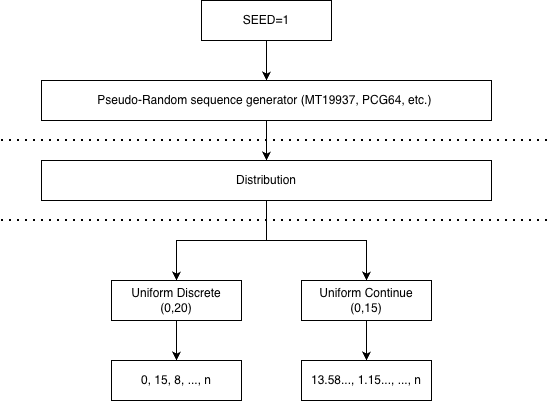
\includegraphics[width=0.65\textwidth]{./random_generation.png}
\caption{Génération de valeurs aléatoires sur environnement informatique}
\end{figure}

\bigskip
\bigskip

Il est important de noter la propriété pseudo-aléatoire du générateur. Ainsi, pour un même “seed”, on obtiendra toujours la même séquence pseudo-aléatoire. Et de fait lors de la création d'une variable aléatoire suivant une distribution particulière, nous aurons toujours la même séquence de nombres pour un même “seed”.

\bigskip

\begin{lstlisting}[language=bash, title=Valeurs générées pour une distribution discrète avec PCG64 et un seed égal à 1]
=== uniform_discrete === 
n:   10, 4 premières et 2 dernières valeurs: [9, 10, 15, 19, ... 5, 6]
n:  100, 4 premières et 2 dernières valeurs: [9, 10, 15, 19, ... 11, 17]
n: 1000, 4 premières et 2 dernières valeurs: [9, 10, 15, 19, ... 20, 14]
n:10000, 4 premières et 2 dernières valeurs: [9, 10, 15, 19, ... 11, 18]
\end{lstlisting}

\subsection{Conditions d'expérimentation}
Le programme créé pour mener les expérimentations de ce TP a été développé en python avec l'aide des librairies:
\begin{itemize}
    \item numpy
    \item matplotlib
\end{itemize}
Le code source est disponible en annexe.

\newpage

% -------------------------------------------------
\section{Distribution uniforme discrète}

\subsection{Description}
\[
P(X = k) = 
\begin{cases} 
\frac{1}{b - a + 1} & \text{si } k \in \{a, a+1, \dots, b\} \\
0 & \text{sinon}
\end{cases}
\]

\subsection{Paramètres}

\begin{itemize}
    \item $a = 0$
    \item $b = 20$
\end{itemize}
\emph{NB: Il y a donc 21 valeurs possibles.}

\bigskip

\subsection{Résultats}

\begin{figure}[H]
\centering
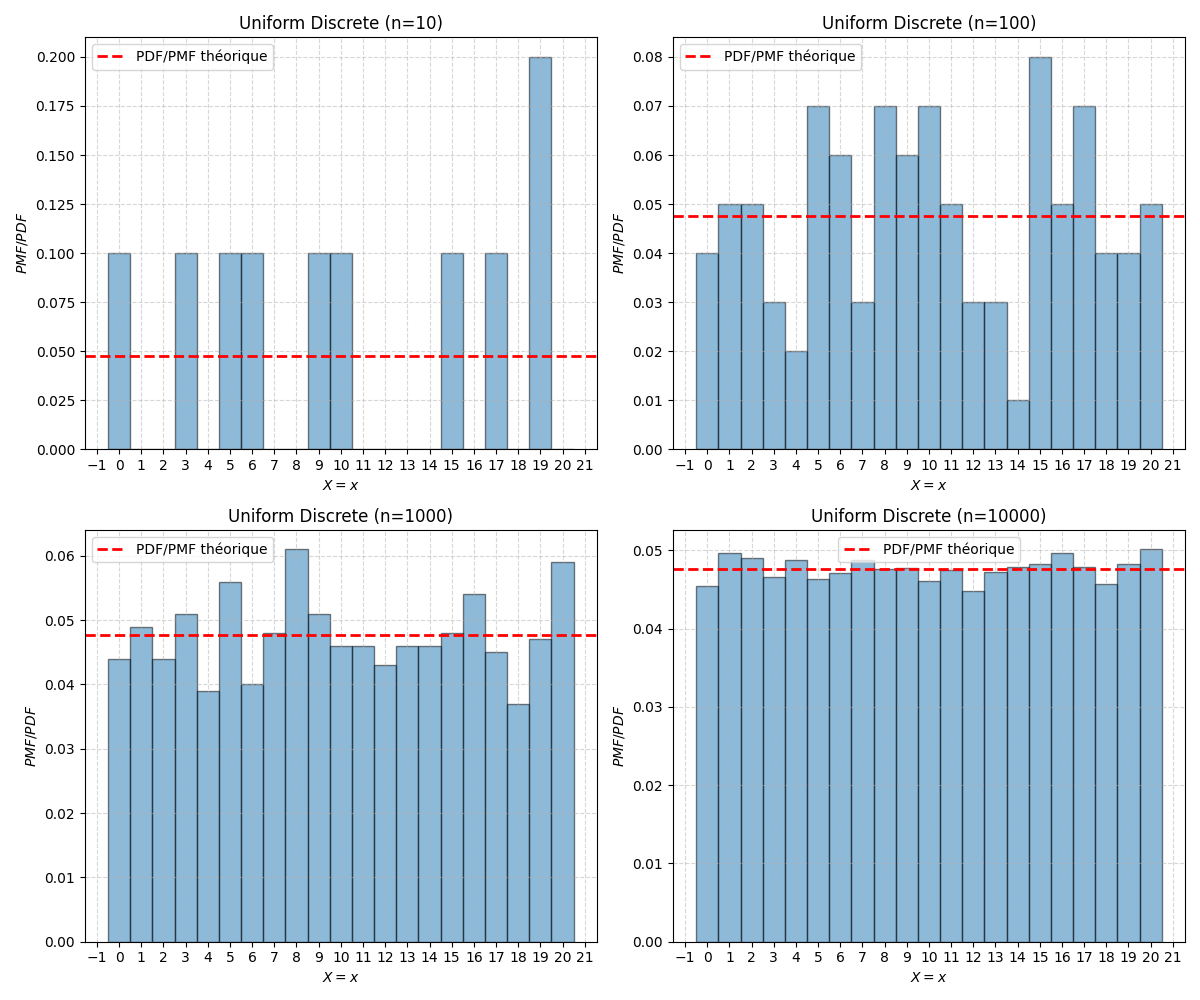
\includegraphics[width=0.95\textwidth]{../uniform_discrete.png}
\caption{Histogramme des valeurs aléatoires pour $n$ tirages, selon une distribution uniforme discrète}
\end{figure}

\newpage

\begin{lstlisting}[language=bash, title=Sortie du terminal pour la distribution uniforme discrète]
=== uniform_discrete ===
n:     10, 5 premières et 5 dernières valeurs: [9, 10, 15, 19, 0 ... 3, 17, 19, 5, 6]
n:     10, Espérance théorique: 10.0, Espérance constatée: 10.3, Delta: 0.3
n:    100, 5 premières et 5 dernières valeurs: [9, 10, 15, 19, 0 ... 15, 1, 3, 11, 17]
n:    100, Espérance théorique: 10.0, Espérance constatée: 10.15, Delta: 0.15
n:   1000, 5 premières et 5 dernières valeurs: [9, 10, 15, 19, 0 ... 2, 1, 16, 20, 14]
n:   1000, Espérance théorique: 10.0, Espérance constatée: 10.06, Delta: 0.061
n:  10000, 5 premières et 5 dernières valeurs: [9, 10, 15, 19, 0 ... 15, 6, 9, 11, 18]
n:  10000, Espérance théorique: 10.0, Espérance constatée: 10.02, Delta: 0.0232
\end{lstlisting}

\subsection{Analyses}
On constate que pour une valeur très faible de tirage l'ensemble des valeurs n'est pas tiré et qu'il existe une grosse différence entre les résultats et la PMF théorique.
Lorsque le nombre de tirage est important l'espérance réelle constatée se rapproche de l'espérance théorique et logiquement le delta diminue.
De même, on observe que l'histogramme, se rapproche de la PMF théorique, au fur et à mesure que le nombre de tirages augmente.

\newpage

% -------------------------------------------------
\section{Distribution uniforme continue}

\subsection{Description}
\[
f(x) = \begin{cases} 
\frac{1}{b - a} & \text{si } a \le x \le b \\ 
0 & \text{sinon} 
\end{cases}
\]

\subsection{Paramètres}

\begin{itemize}
    \item $a = 0.0$
    \item $b = 1.0$
\end{itemize}

\bigskip

\subsection{Résultats}

\begin{figure}[H]
\centering
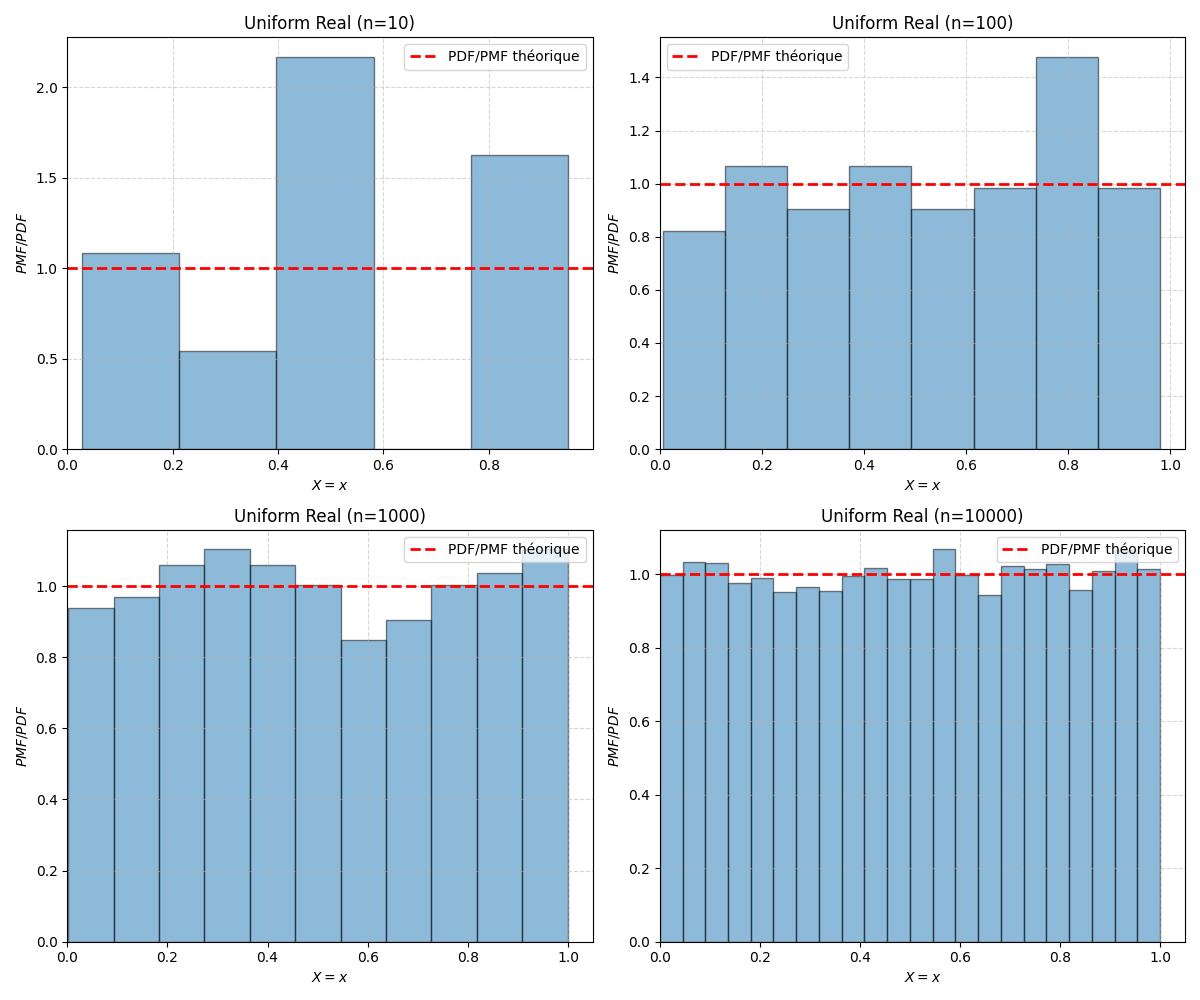
\includegraphics[width=0.95\textwidth]{../uniform_real.png}
\caption{Histogramme des valeurs aléatoires pour $n$ tirages, selon une distribution uniforme continue}
\end{figure}

\newpage

\begin{lstlisting}[language=bash, title=Sortie du terminal pour la distribution uniforme continue]
=== uniform_real ===
n:     10, 5 premières et 5 dernières valeurs: [0.5118, 0.9505, 0.1442, 0.9486, 0.3118 ... 0.4233, 0.8277, 0.4092, 0.5496, 0.02756]
n:     10, Espérance théorique: 0.5, Espérance constatée: 0.5104, Delta: 0.01043
n:    100, 5 premières et 5 dernières valeurs: [0.5118, 0.9505, 0.1442, 0.9486, 0.3118 ... 0.4212, 0.1059, 0.6332, 0.3804, 0.7253]
n:    100, Espérance théorique: 0.5, Espérance constatée: 0.5131, Delta: 0.01307
n:   1000, 5 premières et 5 dernières valeurs: [0.5118, 0.9505, 0.1442, 0.9486, 0.3118 ... 0.5655, 0.9374, 0.01877, 0.8657, 0.9625]
n:   1000, Espérance théorique: 0.5, Espérance constatée: 0.5028, Delta: 0.002805
n:  10000, 5 premières et 5 dernières valeurs: [0.5118, 0.9505, 0.1442, 0.9486, 0.3118 ... 0.4507, 0.6315, 0.1165, 0.3198, 0.4815]
n:  10000, Espérance théorique: 0.5, Espérance constatée: 0.502, Delta: 0.002044
\end{lstlisting}

\subsection{Analyses}
Là encore on constate que pour une valeur très faible de tirage l'ensemble des valeurs n'est pas tiré.
Lorsque le nombre de tirage est important l'espérance réelle constatée se rapproche de l'espérance théorique et logiquement le delta diminue.
De même, on observe que l'histogramme, se rapproche de la PDF théorique, au fur et à mesure que le nombre de tirages augmente.

\newpage

% -------------------------------------------------
\section{Distribution exponentielle}

\subsection{Description}
\[
f(x) = \begin{cases} 
\lambda e^{-\lambda x} & \text{si } x \ge 0 \\ 
0 & \text{si } x < 0 
\end{cases}
\]

\subsection{Paramètres}

\begin{itemize}
    \item $E[x] = 1.0$
\end{itemize}
\emph{donc: $\lambda = 1 / E = 1$}

\bigskip

\subsection{Résultats}

\begin{figure}[H]
\centering
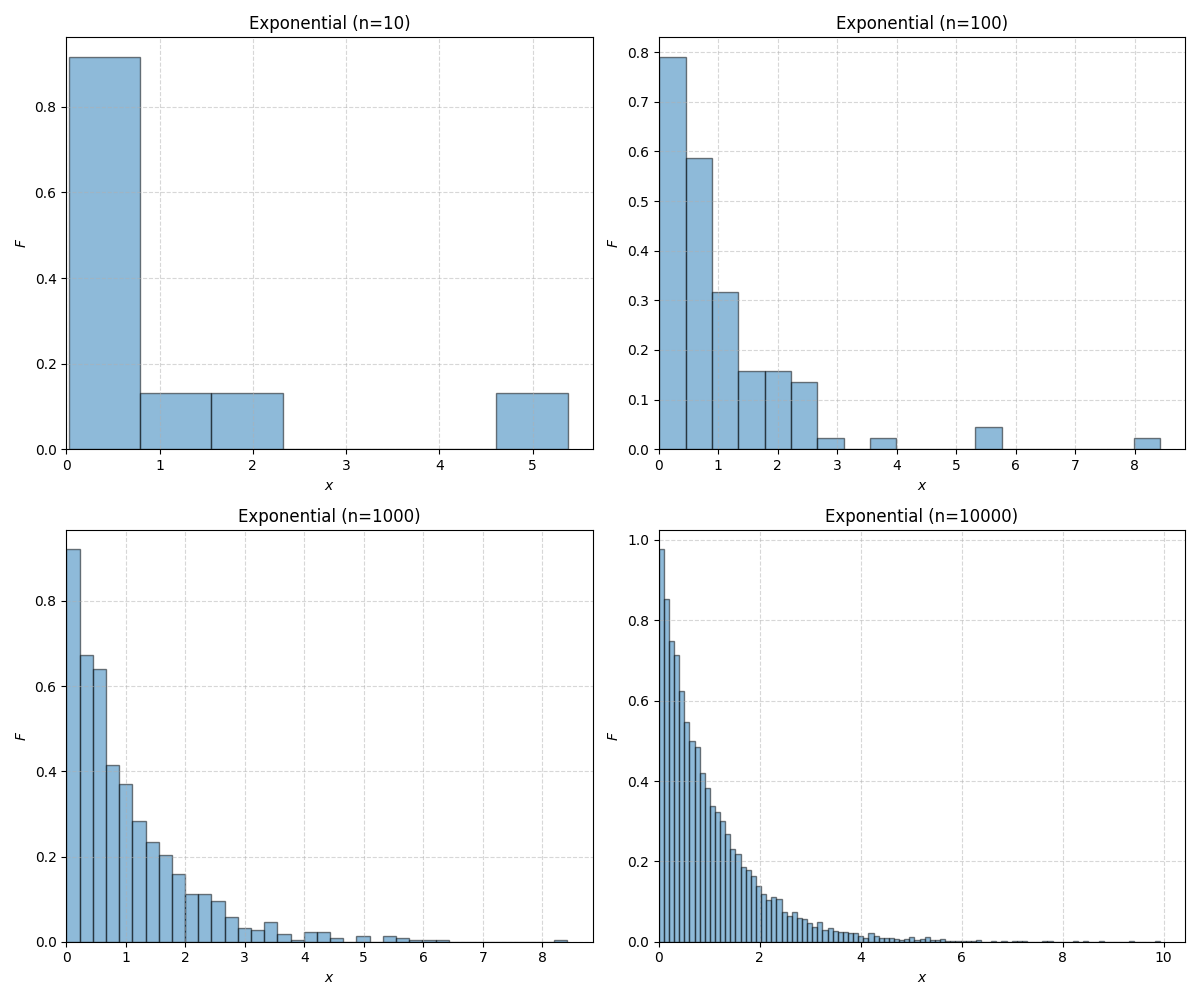
\includegraphics[width=0.95\textwidth]{../exponential.png}
\caption{Histogramme des valeurs aléatoires pour $n$ tirages, selon une distribution exponentielle}
\end{figure}

\newpage

\begin{lstlisting}[language=bash, title=Sortie du terminal pour la distribution exponentielle]
=== exponential ===
n:     10, 5 premières et 5 dernières valeurs: [1.073, 0.3085, 5.375, 0.3664, 0.1154 ... 1.8, 0.4986, 0.5514, 0.02971, 0.7641]
n:     10, Espérance théorique: 1, Espérance constatée: 1.088, Delta: 0.08823
n:    100, 5 premières et 5 dernières valeurs: [1.073, 0.3085, 5.375, 0.3664, 0.1154 ... 0.3736, 1.106, 1.977, 0.627, 0.1648]
n:    100, Espérance théorique: 1, Espérance constatée: 1.038, Delta: 0.03799
n:   1000, 5 premières et 5 dernières valeurs: [1.073, 0.3085, 5.375, 0.3664, 0.1154 ... 0.3449, 1.433, 0.2223, 1.904, 0.1024]
n:   1000, Espérance théorique: 1, Espérance constatée: 1.008, Delta: 0.008393
n:  10000, 5 premières et 5 dernières valeurs: [1.073, 0.3085, 5.375, 0.3664, 0.1154 ... 2.353, 0.1406, 0.91, 0.3969, 0.3701]
n:  10000, Espérance théorique: 1, Espérance constatée: 1.001, Delta: 0.001203
\end{lstlisting}

\subsection{Analyses}
Même s'il est difficile de constater pour un faible nombre de tirages, pour chacun des histogrammes, on observe les caractéristiques de la loi de distribution exponentielle, à savoir :
\begin{itemize}
    \item Une forte probabilité d'avoir une valeur proche de 0
    \item Une décroissance suivant une courbe exponentielle
\end{itemize}
Même si la probabilité d'obtenir un grand nombre est extrêmement faible, on observe que plus notre nombre de tirages augmente, plus nos valeurs maximales augmentent. Cette observation corrobore le fait que la probabilité de tirer un grand nombre reste non nulle. 

\newpage

% -------------------------------------------------
\section{Distribution normale}

\subsection{Description}
\[
f(x) = \frac{1}{\sigma \sqrt{2\pi}} e^{-\frac{1}{2} \left( \frac{x - \mu}{\sigma} \right)^2}
\]

où $\mu$ représente l'espérance (valeur moyenne attendue), et $\sigma$ représente l'écart type.

\subsection{Paramètres}

\begin{itemize}
    \item $\mu = 0.0$
    \item $\sigma = 1.0$
\end{itemize}

\bigskip

\subsection{Résultats}

\begin{figure}[H]
\centering
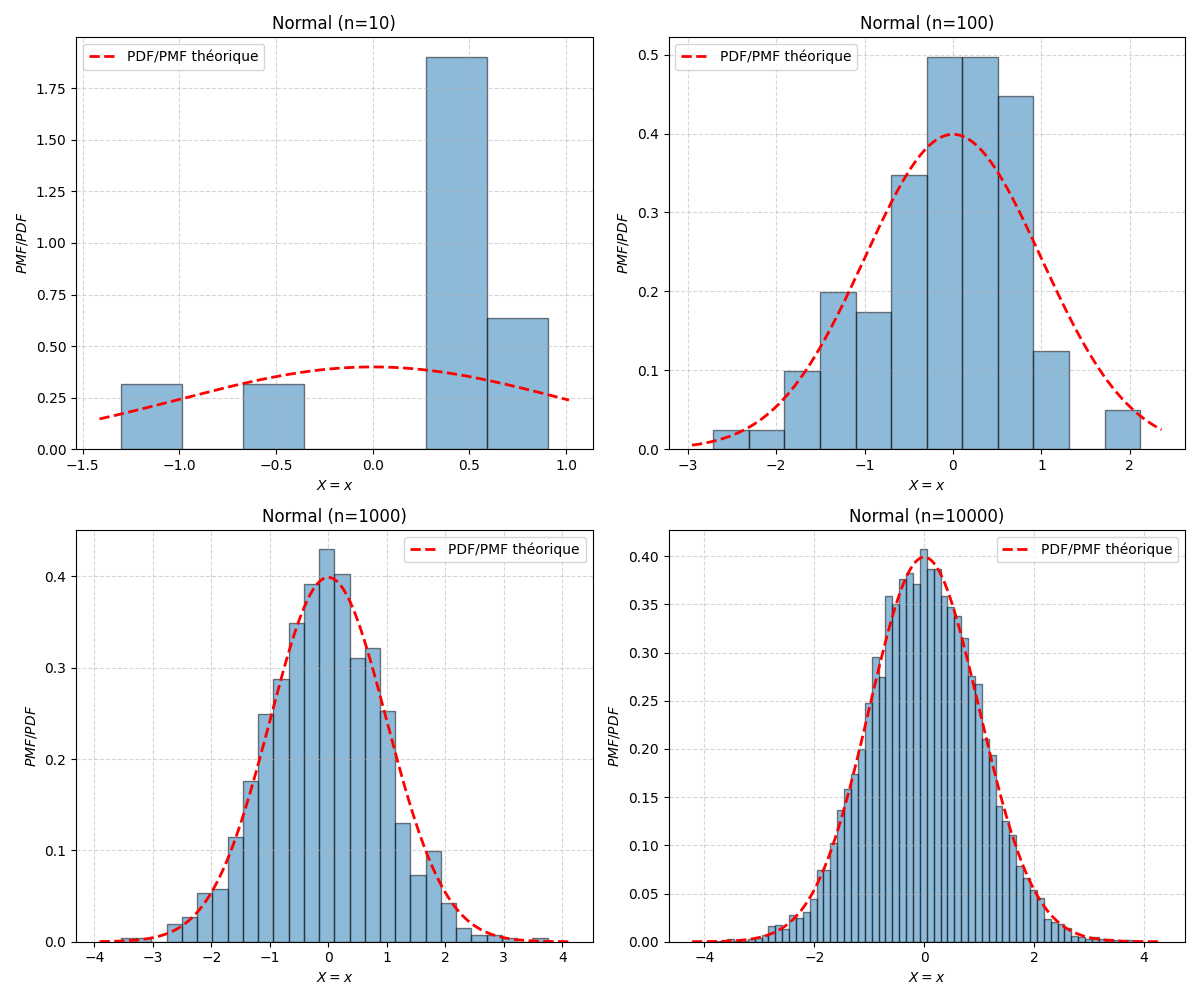
\includegraphics[width=0.95\textwidth]{../normal.png}
\caption{Histogramme des valeurs aléatoires pour $n$ tirages, selon une distribution normale}
\end{figure}

\newpage

\begin{lstlisting}[language=bash, title=Sortie du terminal pour la distribution normale]
=== normal ===
n:     10, 5 premières et 5 dernières valeurs: [0.3456, 0.8216, 0.3304, -1.303, 0.9054 ... 0.4464, -0.537, 0.5811, 0.3646, 0.2941]
n:     10, Espérance théorique: 0, Espérance constatée: 0.2249, Delta: 0.2249
n:    100, 5 premières et 5 dernières valeurs: [0.3456, 0.8216, 0.3304, -1.303, 0.9054 ... -2.251, -0.1387, 0.033, -1.425, 0.3328]
n:    100, Espérance théorique: 0, Espérance constatée: -0.07361, Delta: -0.07361
n:   1000, 5 premières et 5 dernières valeurs: [0.3456, 0.8216, 0.3304, -1.303, 0.9054 ... -0.3388, -2.418, -0.0762, -0.3971, 0.275]
n:   1000, Espérance théorique: 0, Espérance constatée: -0.05425, Delta: -0.05425
n:  10000, 5 premières et 5 dernières valeurs: [0.3456, 0.8216, 0.3304, -1.303, 0.9054 ... 1.425, 1.601, 0.3013, -0.7713, 0.1855]
n:  10000, Espérance théorique: 0, Espérance constatée: -0.01091, Delta: -0.01091
\end{lstlisting}

\subsection{Analyses}

On constate que pour une valeur très faible de tirage l'ensemble des valeurs n'est pas tiré.
Plus on augmente le nombre de tirages, plus la forme de l'histogramme prend rapidement une forme de cloche quasi symétrique, centrée autour de notre valeur moyenne, caractéristique de la loi normale.
On constate, même avec un nombre de tirages relativement faible, qu'on retrouve la règle empirique de répartition de la loi normale : 

\begin{itemize}
\item 68 \% des données se situent à moins de 1 écart-type de la moyenne.
\item 95 \% des données se situent à moins de 2 écarts-types de la moyenne.
\item 99,7 \% des données se situent à moins de 3 écarts-types de la moyenne.
\end{itemize}

Cependant, pour un nombre de tirage trop faible (ici 10), on constate que notre tirage ne nous amène pas à obtenir notre valeur moyenne attendue.

\newpage

% -------------------------------------------------
\section{Distribution binomiale}

\subsection{Description}
\[
P(X = k) = \begin{cases} 
\binom{n}{k} p^k (1-p)^{n-k} & \text{si } k \in \{0, 1, \dots, n\} \\ 
0 & \text{sinon} 
\end{cases}
\]

\subsection{Paramètres}

\begin{itemize}
    \item $p = 0.5$
    \item $n = 10$
\end{itemize}

\bigskip

\subsection{Résultats}

\begin{figure}[H]
\centering
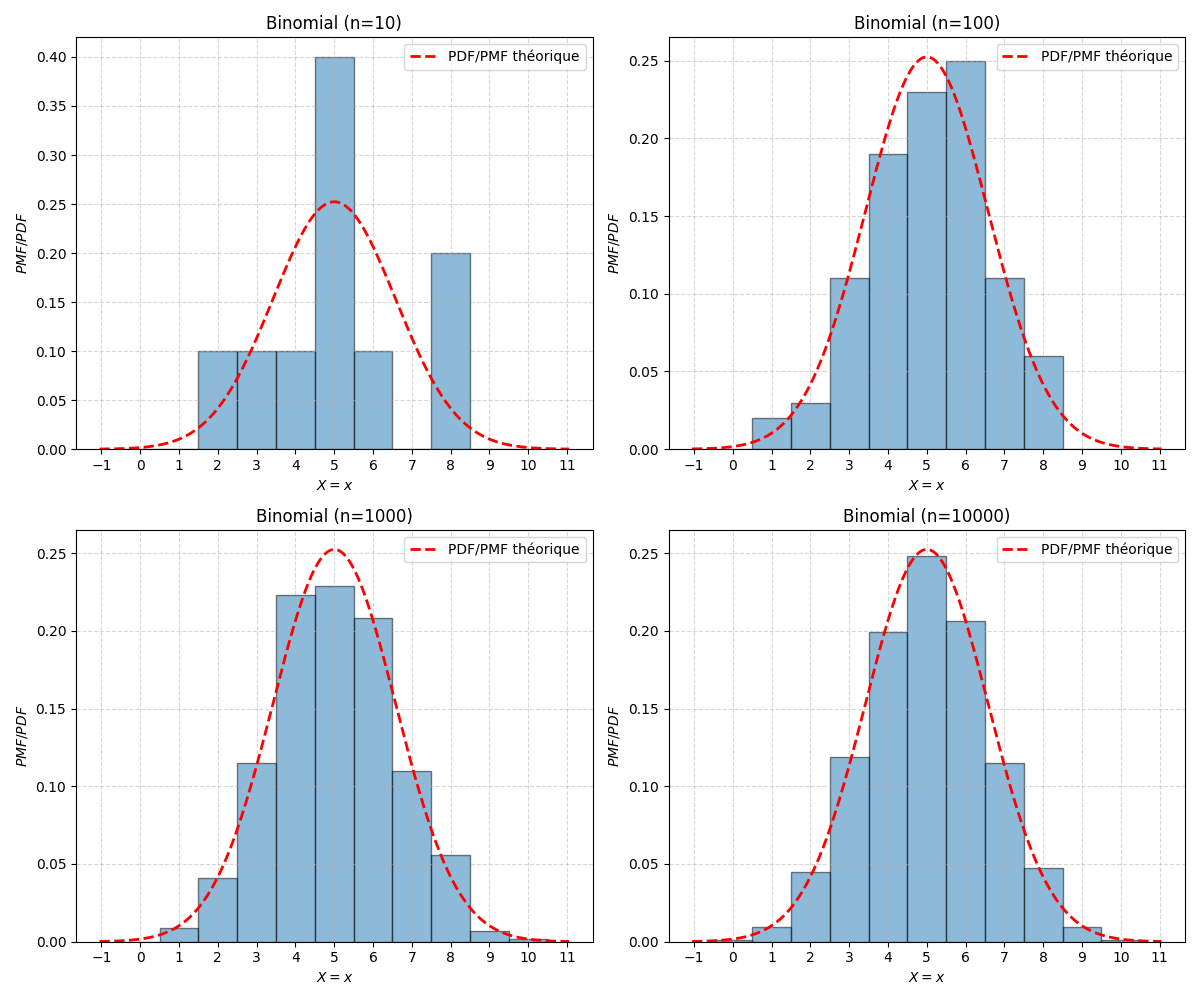
\includegraphics[width=0.95\textwidth]{../binomial.png}
\caption{Histogramme des valeurs aléatoires pour $n$ tirages, selon une distribution binomiale}
\end{figure}

\newpage

\begin{lstlisting}[language=bash, title=Sortie du terminal pour la distribution binomiale]
=== binomial ===
n:     10, 5 premières et 5 dernières valeurs: [5, 8, 3, 8, 4 ... 5, 6, 5, 5, 2]
n:     10, Espérance théorique: 5.0, Espérance constatée: 5.1, Delta: 0.1
n:    100, 5 premières et 5 dernières valeurs: [5, 8, 3, 8, 4 ... 5, 3, 6, 5, 6]
n:    100, Espérance théorique: 5.0, Espérance constatée: 5.07, Delta: 0.07
n:   1000, 5 premières et 5 dernières valeurs: [5, 8, 3, 8, 4 ... 5, 7, 2, 7, 8]
n:   1000, Espérance théorique: 5.0, Espérance constatée: 5.022, Delta: 0.022
n:  10000, 5 premières et 5 dernières valeurs: [5, 8, 3, 8, 4 ... 5, 6, 3, 4, 5]
n:  10000, Espérance théorique: 5.0, Espérance constatée: 5.007, Delta: 0.0067
\end{lstlisting}

\subsection{Analyses}

Comme la probabilité $p$ choisie ici est égale à 0.5, on s'attend à obtenir majoritairement 5 “succès” pour 10 tirages.
Pour autant, nous observons que la probabilité que cette valeur soit différente de 5 reste non nulle, comme le définit la loi binomiale.
De plus, on constate que lorsque le nombre de tirages devient très grand, on voit se dessiner l'approximation de la loi binomiale définie par:

\[
f(x) \approx \frac{1}{\sqrt{2\pi np(1-p)}} e^{-\frac{(x-np)^2}{2np(1-p)}}
\]

\bigskip
\bigskip
\bigskip


% -------------------------------------------------
\section{Conclusion}

À travers ce TP, nous avons pu observer et mettre évidence les principales caractéristiques de quelques distributions de variables aléatoires. 

Nous avons observé à travers les histogrammes que, pour toutes les distributions étudiées, plus le nombre de tirages est grand, plus les résultats se rapprochent des valeurs théoriques attendues. La diminution de l'écart entre les valeurs théoriques attendues, et les valeurs observées, à mesure que le nombre de tirages augmente, met en évidence la loi des grands nombres, vue en cours. 

\newpage

% -------------------------------------------------
\section*{Annexe : Code source}

\begin{lstlisting}[language=Python,caption=Code source du programme développé]
import numpy as np
import matplotlib.pyplot as plt
from matplotlib.ticker import MultipleLocator

# ========================================================
# CONSTANTS

SEED = 1
N_VALUES = [10, 100, 1000, 10000]


# ========================================================
# COMMONS


def init_axes():
    _, axes = plt.subplots(
        int(np.sqrt(len(N_VALUES))), int(np.sqrt(len(N_VALUES))), figsize=(12, 10)
    )
    axes = axes.ravel()
    return axes


def draw_on_axe(
    axe, x, n, title, bins="auto", use_int_x_axes=False, start_at_zero=True, func=None
):
    axe.hist(x, bins=bins, edgecolor="black", alpha=0.5, density=True)
    axe.set_title(f"{title} (n={n})")
    axe.set_xlabel("$X = x$")
    axe.set_ylabel("$PMF/PDF$")
    axe.grid(True, linestyle="--", alpha=0.5)
    if use_int_x_axes:
        axe.xaxis.set_major_locator(MultipleLocator(1))
    if start_at_zero:
        axe.set_xlim(left=0)
        axe.set_ylim(bottom=0)

    if func is not None:
        x_vals = np.linspace(axe.get_xlim()[0], axe.get_xlim()[1], 1000)
        y_vals = func(x_vals)

        if isinstance(y_vals, float) or isinstance(y_vals, int):
            axe.axhline(
                y=y_vals,
                color="red",
                linestyle="--",
                linewidth=2,
                label="PDF/PMF théorique",
            )
        else:
            axe.plot(
                x_vals,
                y_vals,
                color="red",
                linestyle="--",
                linewidth=2,
                label="PDF/PMF théorique",
            )
        axe.legend()


def format_value(val):
    return str(val) if val.is_integer() else f"{val:.4}"


def print_x(x, n, esp):
    print(
        f"n: {n:6}, 5 premières et 5 dernières valeurs: [{', '.join([format_value(val) for val in x[:5]])} ... {', '.join([format_value(val) for val in x[-5:]])}]"
    )
    real = np.mean(x)
    delta = real - esp
    print(
        f"n: {n:6}, Espérance théorique: {format_value(esp)}, Espérance constatée: {format_value(real)}, Delta: {format_value(delta)}"
    )


# ========================================================
# DISTRIBUTIONS


def uniform_discrete():
    axes = init_axes()
    print("=== uniform_discrete ===")
    for i, n in enumerate(N_VALUES):
        MIN = 0
        MAX = 20
        rng = np.random.default_rng(seed=SEED)
        x = rng.integers(low=MIN, high=MAX + 1, size=n)
        uniform_pmf = lambda t_x: 1 / (MAX - MIN + 1)
        draw_on_axe(
            axes[i],
            x,
            n,
            "Uniform Discrete",
            bins=np.arange(-0.5, MAX + 1 + 0.5, 1),
            start_at_zero=False,
            use_int_x_axes=True,
            func=uniform_pmf,
        )
        print_x(x, n, (MIN + MAX) / 2)
    plt.tight_layout()
    plt.savefig("uniform_discrete.png")


def uniform_real():
    axes = init_axes()
    print("\n=== uniform_real ===")
    for i, n in enumerate(N_VALUES):
        rng = np.random.default_rng(seed=SEED)
        # By default, rng.uniform return values in range [0.0;1.0] (include)
        x = rng.uniform(size=n)
        MAX = 1
        MIN = 0
        uniform_pmf = lambda t_x: 1 / (MAX - MIN)
        draw_on_axe(axes[i], x, n, "Uniform Real", func=uniform_pmf)
        print_x(x, n, (0.0 + 1.0) / 2)
    plt.tight_layout()
    plt.savefig("uniform_real.png")


def exponential():
    axes = init_axes()
    print("\n=== exponential ===")
    for i, n in enumerate(N_VALUES):
        AVG = 1
        LAMBDA = 1 / AVG
        # More AVG is high, more the distibution decrease quickly
        rng = np.random.default_rng(seed=SEED)
        x = rng.exponential(scale=LAMBDA, size=n)
        exp_pdf = lambda t_x: LAMBDA * np.exp(-LAMBDA * t_x)
        draw_on_axe(axes[i], x, n, "Exponential", func=exp_pdf)
        print_x(x, n, AVG)
    plt.tight_layout()
    plt.savefig("exponential.png")


def normal():
    axes = init_axes()
    print("\n=== normal ===")
    for i, n in enumerate(N_VALUES):
        MU_AVG = 0
        SIGMA_VAR = 1
        rng = np.random.default_rng(seed=SEED)
        x = rng.normal(loc=MU_AVG, scale=SIGMA_VAR, size=n)
        normal_pdf = lambda t_x: np.exp(-(((t_x - MU_AVG) / SIGMA_VAR) ** 2) / 2) / (
            SIGMA_VAR * np.sqrt(2 * np.pi)
        )
        draw_on_axe(axes[i], x, n, "Normal", start_at_zero=False, func=normal_pdf)
        print_x(x, n, MU_AVG)
    plt.tight_layout()
    plt.savefig("normal.png")


def binomial():
    axes = init_axes()
    print("\n=== binomial ===")
    for i, n in enumerate(N_VALUES):
        N = 10
        P = 0.50
        Q = 1 - P
        rng = np.random.default_rng(seed=SEED)
        x = rng.binomial(p=P, n=N, size=n)
        normal_approx = lambda t_x: (1 / np.sqrt(2 * np.pi * N * P * Q)) * np.exp(
            -0.5 * ((t_x - N * P) ** 2) / (N * P * Q)
        )

        draw_on_axe(
            axes[i],
            x,
            n,
            "Binomial",
            bins=np.arange(-0.5, N + 1 + 0.5, 1),
            use_int_x_axes=True,
            start_at_zero=False,
            func=normal_approx,
        )
        print_x(x, n, N * P)
    plt.tight_layout()
    plt.savefig("binomial.png")


# ========================================================
# MAIN
if __name__ == "__main__":
    uniform_discrete()
    uniform_real()
    exponential()
    normal()
    binomial()

\end{lstlisting}

\end{document}
